\documentclass{report}

\usepackage[utf8]{inputenc}
\usepackage[a4paper, total={6in, 8in}]{geometry}
\usepackage{amsmath}
\usepackage{amsthm}
\usepackage{fancyhdr}
\usepackage{natbib}
\usepackage{mathpazo}

\usepackage{pgf,tikz}
\usepackage{mathrsfs}
\usetikzlibrary{arrows}

\usepackage{graphicx}
\graphicspath{ {images/}{drafts/} }
\usepackage{caption}

\usepackage{enumerate}
\usepackage{type1cm}
\usepackage{exercise,chngcntr}

\newenvironment{solution}
  {\begin{proof}[Solution]}
  {\end{proof}}

\newenvironment{sketch}
  {\begin{proof}[Sketch]}
  {\end{proof}}
  
\pagestyle{fancy}
\fancyhf{}
\rhead{\rightmark}
\rfoot{\thepage}

\begin{document}
\counterwithin{Exercise}{section}

\setcounter{chapter}{7}
\chapter{Euclidean Spaces}
\thispagestyle{empty}
\newpage

% === Section 8.1 ===
\section{Algebraic Structure}

\setcounter{Exercise}{1}
% === Exercise 8.1.2 ===
\begin{Exercise}
\begin{enumerate}[a)]
\item 
\begin{proof}
Consider 
\begin{align*}
\|v\| 
&= \left\| \frac{(a\cdot b)c+(a\cdot c)b+(c\cdot b)a}{3} \right\| \\
&= \frac{1}{3} \left( \|a\cdot b\| \|c\| + \|a\cdot c\| \|b\|+\|c\cdot b\| \|a\|\right) \\
&\leq \|a\|\|b\| \|c\| \\
&\leq 1,
\end{align*}
hence $v\in B$ as promised.
\end{proof}

\item
\begin{proof}
For all $c, d\in \mathbb{R}^n$,
\begin{align*}
|a\cdot c - b\cdot d|
&= |a\cdot c - a\cdot b + a\cdot b - b\cdot d| \\
&= | a(c-b) + b(a-d) | \\
&\leq | a(c-b) | + | b(a-d) | \\
&= \|a\|\|b-c\| + \|b\|\|a-d\| \\
&\leq \|b-c\| + \|a-d\|
\end{align*}
\end{proof}

\item
\begin{proof}
\begin{align*}
\sqrt{|a\cdot (b \times c) |^2 + |a\cdot b|^2}
&= \sqrt{|(a \times b) \cdot c|^2 + |a\cdot b|^2} \\
&= \sqrt{\|a\times b\|^2 \|c\|^2 + |a\cdot b|^2} \\
&\leq \sqrt{\|a\times b\|^2 + |a\cdot b|^2} \\
&= \sqrt{(a\cdot a)(b\cdot b) - (a\cdot b)^2 + |a\cdot b|^2} \\
&= \sqrt{(\|a\|^2 \|b\|^2 - |a\cdot b|^2 + |a\cdot b|^2} \\
&= \sqrt{\|a\|^2 \|b\|^2} \\
&\leq 1
\end{align*}
\end{proof}
\end{enumerate}
\end{Exercise}

\vspace{12pt}

\setcounter{Exercise}{8}
% === Exercise 8.1.9 ===
\begin{Exercise}
\begin{proof}
Since $|a_k|, |b_k| \geq 0$, by the Arithmetic-Geometric mean Inequality, we consider
$$\sum_{k=1}^{\infty} |a_k b_k|
\leq \sum_{k=1}^{\infty} \frac{a_k^2+b_k^2}{2}
= \frac{1}{2}\left(\sum_{k=1}^{\infty} a_k^2 + \sum_{k=1}^{\infty} b_k^2 \right).$$
Since the rightest hand converges by hypotheses. Moreover, by the Comparison Test, we conclude $$\sum_{k=1}^{\infty}a_k b_k$$ converges absolutely.
\end{proof}
\end{Exercise}


% === Section 8.2 ===
\section{Planes and Linear Transformation}

\setcounter{Exercise}{3}
% === Exercise 8.2.4 ===
\begin{Exercise}
\begin{enumerate}[a)]
\item 
\begin{solution}
$$ T = \begin{bmatrix}
  0 & 0 & 0 & 0 \\
  1 & 1 & 0 & 0 \\
  1 & 0 & -1 & 0 \\
  1 & 1 & 0 & 1
\end{bmatrix}.
$$
\end{solution}

\item
\begin{solution}
$$ T = \begin{bmatrix}
1 & -1 & 1
\end{bmatrix}.
$$
\end{solution}

\item
\begin{solution}
$$ T = \begin{bmatrix}
1 & 0 & \cdots & 0 & -1 \\
-1 & 0 & \cdots & 0 & 1
\end{bmatrix}_{2\times n}.
$$
\end{solution}
\end{enumerate}
\end{Exercise}

\vspace{12pt}

\setcounter{Exercise}{10}
% === Exercise 8.2.11 ===
\begin{Exercise}
\begin{enumerate}[a)]
\item 
\begin{proof}
Let $x \in \mathbb{R}^n$ with $\|x\|=1$, then
$$ \| T(x) \|
\leq \|T\| \|x\|
= \|T\|.$$
By definition of $M_1$, we conclude $M_1 \leq \|T\|$.
\end{proof}

\item
\begin{proof}
Since $T$ is linear, for $x \neq 0$,
$$ \frac{\|T(x)\|}{\|x\|}
= \left\| T\left( \frac{x}{\|x\|} \right) \right\|
\leq M_1.$$ where $ \| \frac{x}{\|x\|} \| = 1$.
\end{proof}

\item 
\begin{proof}
From part a), we know $M_1 \leq \|T\|$. And from part b), taking the supremum of left hand, then by definition of $\|T\|$, we also know $$\sup_{x\neq 0}\frac{\|T(x)\|}{\|x\|} = \|T\| \leq M_1.$$
Hence we have $M_1 = \|T\|$ at first.

\vspace{1ex}

For any $C>0$, considering $$\|T(x)\|\leq C\|x\|$$, we have $\|T\| \leq C$. Then taking the infimum of right hand, we know $\|T\| \leq M_2$. On the other hand, $\|T\|$ is finite and $$\|T(x)\| \leq \|T\|\|x\|.$$ Hence $M_2\leq \|T\|$, then we have $M_2 = \|T\|$.

\vspace{1ex}

Finally, together all the discussions, we conclude $M_1 = M_2 = \|T\|$ as promised.
\end{proof}
\end{enumerate}
\end{Exercise}


% === Section 8.3 ===
\section{Topology of $\mathbb{R}^n$}

\setcounter{Exercise}{3}
% === Exercise 8.3.4 ===
\begin{Exercise}
\begin{enumerate}[a)]
\item
\begin{sketch}
See the handwriting.

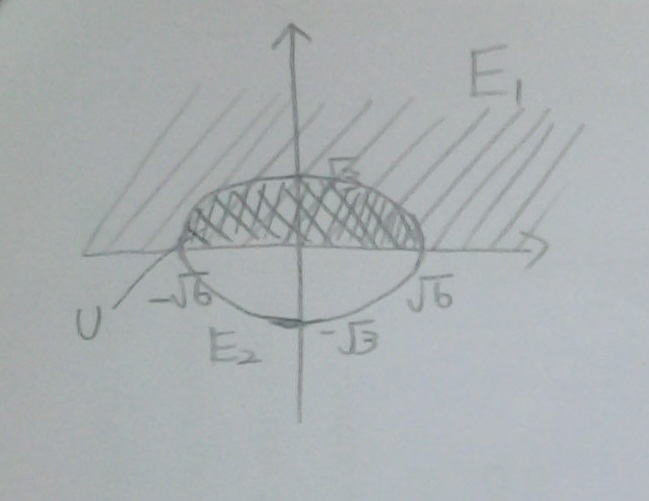
\includegraphics[width=6cm]{fig_8_3_4_a}

\end{sketch}

\item
\begin{solution}
Consider $E_1$ and $E_2$ are subsets of $\mathbb{R}^2$. Since $E_1$ is closed, hence $U=E_1\cap E_2$ is $\mathbf{relatively\ open}$ in $E_1$.
\end{solution}

\item
\begin{solution}
Since $E_2$ is open, hence $U=E_1\cap E_2$ is $\mathbf{relatively\ closed}$ in $E_2$.
\end{solution}
\end{enumerate}
\end{Exercise}

\vspace{12pt}

\setcounter{Exercise}{5}
% === Exercise 8.3.6 ===
\begin{Exercise}
\begin{enumerate}[a)]
\item
\begin{proof}
$(\Longrightarrow)$
Since $C$ is relatively closed in $E$, then by definition, there exists a closed set $B$ such that $C=E\cap B$. Because $E$ and $B$ are closed, we conclude $C$ is closed.

$(\Longleftarrow)$
Since $C\subseteq E$ implies $C=C\cap E$, and we know $C$ and $E$ are closed by hypotheses. By definition, we conclude $C$ is relatively closed in $E$.
\end{proof}

\item
\begin{proof}
$(\Longrightarrow)$
Since $C$ is relatively closed in $E$, there exists a closed set $B$ such that $C=E\cap B$.

Consider
$$
C\backslash E 
= C\cap E^c 
= E\cap \left(E\cap B \right)^c 
= E\cap \left( E^c\cup B^c \right) 
= \left( E\cap E^c\right) \cup \left( E \cap B^c\right)
= E\cap B^c.
$$
Since $B^c$ is open, we conclude $E\backslash C$ is relatively open in $E$.

$(\Longleftarrow)$
Since $E\backslash C$ is relatively open in $E$, there exists an open set $A$ such that $E\backslash C = E\cap A$. Consider
\begin{align*}
C
&= E\cap C
= \left( E\cap E^c \right) \cup \left(E \cap C\right)
= E\cap \left( E^c \cup C \right) \\
&= E\cap \left( E\cap C^c \right)^c
= E\cap \left( E\cap A \right)^c
= E\cap \left( E^c \cup A^c \right) \\
&= E \cap A^c.
\end{align*}
Since $A^c$ is closed, we conclude $C$ is relatively closed in $E$.
\end{proof}

\end{enumerate}
\end{Exercise}

\vspace{12pt}

% === Exercise 8.3.7 ===
\begin{Exercise}
\begin{enumerate}[a)]
\item
\begin{proof}
Suppose $A\cup B$ is $\mathbf{not}$ connected. i.e., there exists nonempty sets $U$, $V$ are relatively open in $A\cup B$ such that $U\cap V=\phi$ and $U\cup V=A\cup B$.
\begin{enumerate}
\item [$\mathbf{Case\ 1.}$] 
$A\cap U\neq \phi$ and $B\cap V\neq \phi$.

\vspace{1ex}

Set $U' := A\cap U$ and $V' := A\cap V$. We claim $U'$ and $V'$ separate $A\cup B$. \\
Consider $U'\cap V' = (A\cap U)\cap (A\cap V) = A\cap (U\cap V) = A\cap \phi = \phi.$
Then since $U$ is relatively open in $A\cup B$, there exists an open set $G$ such that $U = (A\cup B)\cap G$. Moreover, 
$$
U'
= A\cap U
= A\left( (A\cup B)\cap G \right)
= A\cap G.
$$
Hence $U'$ is relatively open in $A$ so is $V'$ with a similar argument.
Finally, we verify
$$
U'\cup V'
= (A\cap U)\cup(A\cap V)
= A\cap (U\cup V)
= A\cap (A\cup B)
= A.
$$
By definition, we conclude $U'$ and $V'$ separate $A$ which implies $A$ is not connected. This leads to a contradiction with hypotheses that $A$ is connected.

\item [$\mathbf{Case\ 2.}$]
$A\cap U = \phi$ or $B\cap V = \phi$.

\vspace{1ex}

W.L.O.G., we assume $A\cap U = \phi$. Consider
\begin{flalign*}
& A\cup B = U\cup V &\\
\implies& U\cap(A\cup B) = U\cap(U\cup V) &\\
\implies& (U\cap A)\cup (U\cap B) = U &\\
\implies& \phi\cup(U\cap) = U &\\
\implies& U\cap B = U &\\
\implies& U \subseteq B. &
\end{flalign*}
Set $B_1 := B\cap U$ and $B_2 := B\cap V$.
We consider
\begin{align*}
B_1\cup B_2
&= (B\cap U) \cup (B\cap V) \\
&= B\cap(U\cup U) \\
&= B\cap(A\cup B) \\
&= B.
\end{align*}
Moreover, with a similar argument from $\mathbf{Case\ 1.}$, we also know $B_1$ and $B_2$ are relatively open in $B$. By the way, $U = U\cap B = B_1 \neq \phi$. Then we should discuss whether $B_2 = \phi$ or not.

If $B_2 \neq \phi$, then since $B_2 = B\cap V$, we claim $B_1$ and $B_2$ separate $B$ by definition.
Otherwise $B_2 = \phi$, then continue to consider
\begin{flalign*}
& A\cup B = U\cup V &\\
\implies& A\cap(A\cup B) = A\cap(U\cup V) &\\
\implies& A = (A\cap U)\cup (A\cap V) &\\
\implies& A = A\cap V & \\
\implies& A \subseteq V. &
\end{flalign*}
Since $B\cap V = \phi$ implies $V \subseteq B^c$, so $A \subseteq B^c$. We conclude $A\cap B = \phi$ which leads to a contradiction with hypotheses that $A\cap B\neq \phi$.

A similar argument proves the condition $B\cap V = \phi$. 
\end{enumerate}
Finally, we conclude $A\cap B$ is connected under the hypotheses as promised.
\end{proof}

\item
\begin{proof}
Denote $$E_k := \bigcup_{i=1}^{k}E_{n_i}.$$
where $n_i\in A \mbox{ for } i=1,2,\cdots,k$.
We pick $n_1\in A$ arbitrarily, then $E_1 = E_{n_1}$ is connected by hypotheses.

Assume for $n=k$, $E_k$ is connected. Then for $n=k+1$, we
pick $n_{k+1}\in A$ arbitrarily, then we know $E_k$ and $E_{n_{k+1}}$ are connected sets. Since $\cap_{\alpha\in A}E_{\alpha} \neq \phi$, it follows that $E_k \cap E_{n_{k+1}} \neq \phi$. From part a), we have $E_k \cup E_{n_{k+1}} = E_{k+1}$ is also connected.
By induction, we know $E_k$ is connected for all $k\in\mathbb{N}$ which implies
$$
E = \bigcup_{\alpha\in A} E_{\alpha}
$$ is connected.
\end{proof}

\item
\begin{proof}
Since a subset of $\mathbb{R}$ is connected if and only if $E$ is an interval, we suppose $A = [a_1, b_1]$ and $B = [a_2, b_2]$. Since $A\cap B \neq \phi$, we discuss all conditions which are fulfilled.
\begin{enumerate}
\item [$\mathbf{Case\ 1.}$]
$a_1 \leq b_1$ and $b_1 \leq a_2 < b_2$

where $A\cap B = [b1, a2] \neq \phi$. Then $A\cup B = [a_1, b_2]$ is an interval, so is connected.

\item [$\mathbf{Case\ 2.}$]
$a_1 \leq b_1$ and $a_2 \geq b_2$.

where $A\cap B = [b1, b2] \neq \phi$. Then $A\cup B = [a_1, a_2]$ is an interval, so is connected.

\item [$\mathbf{Case\ 3.}$]
$b_1 \leq a_1$ and $a_1 \leq b_2 < a_2$.

where $A\cap B = [a1, b2] \neq \phi$. Then $A\cup B = [b_1, a_2]$ is an interval, so is connected.

\item [$\mathbf{Case\ 4.}$]
$b_1 \leq a_1$ and $b_2 \geq a_2$.

where $A\cap B = [a1, a2] \neq \phi$. Then $A\cup B = [b_1, b_2]$ is an interval, so is connected.
\end{enumerate}
Hence, $A\cap B$ is always connected as promised.
\end{proof}

\item
\begin{proof}
The counter-example is that two subsets of $\mathbb{R}^2$ are supposed as following, 
\begin{align*}
A &:= \{(x,y) : -1\leq x \leq 1, -|x| \leq y \leq |x|\} \\
B &:=\{(x,y) : -1 \leq x \leq 1, -1 \leq y \leq 1\}\backslash\{(0,0)\}
\end{align*}
where $A\cap B = \{(x, y): -1 \leq x \leq 1, -|x| \leq y \leq |x|\} \backslash \{(0,0)\} \neq \phi.$

We can pick $U := \{(x,y):x<0\}$ and $V := \{(x,y):x>0\}$ to separate $A\cap B$, so $A\cap B$ is not connected.
\end{proof}

\end{enumerate}
\end{Exercise}

\vspace{12pt}

% === Exercise 8.3.8 ===
\begin{Exercise}
\begin{enumerate}[a)]
\item
\begin{proof}
$(\Longrightarrow)$

For any $x\in V$, since $V$ is open, there exists $r(x)>0$ such that $B_{r(x)}(x)\subset V$. Then $$V\subset \bigcup_{x\in V}B_{r(x)}(x)\subset \bigcup_{x\in V}V = V.$$
Hence $V=\bigcup_{\alpha\in A}B_{\alpha}$.

\vspace{2ex}

$(\Longleftarrow)$

We replace the notation $B_{\alpha}$ with $V_{\alpha}$. Let $x\in\bigcup_{\alpha\in A} V_{\alpha}$. Then $x\in V_{\alpha}$ for some $\alpha\in A$. Since $V_{\alpha}$ is open, it follows that there is an $r>0$ such that $B_{r}(x)\subseteq V_{\alpha}$. Thus $B_r(x)\subseteq \bigcup_{\alpha\in A}V_{\alpha} = V$ is open. 
\end{proof}

\item
\begin{solution}
We interpret the statement as "Prove that $V$ is $\mathbf{closed}$ if and only if there is a collection of $\mathbf{closed}$ balls $\{B_{\alpha}:\alpha\in A\}$ such that $V=\bigcup_{\alpha\in A}B_{\alpha}$".

So let $B_k = [\frac{1}{k+1}, \frac{k}{k+1}]$ is closed for each $k\in\mathbb{N}$. Then we know $$\bigcup_{k\in\mathbb{N}}B_k = (0, 1)$$ is open. Hence the result will fail.
\end{solution}
\end{enumerate}
\end{Exercise}

\vspace{12pt}

% === Exercise 8.3.9 ===
\begin{Exercise}
\begin{enumerate}[a)]
\item
\begin{proof}
Since $E$ is closed, then $E^c$ is open. So for any $a\in E^c$, there exists $r>0$ such that $B_r(a)\subseteq E^c$. For any $x\in E$, since $x\notin B_r(a)$, then $$ \| x-a \| \geq r > 0.$$
It follows that $$ \inf_{x\in E} \| x-a \| > 0.$$
\end{proof}
\end{enumerate}
\end{Exercise}


% === Section 8.4 ===
\section{Interior, Closure, and Boundary}

\setcounter{Exercise}{1}
% === Exercise 8.4.2 ===
\begin{Exercise}
\begin{enumerate}[a)]
\item
\begin{sketch} 
See the Figure \ref{fig:8.4.2_a}.

\begin{minipage}[h]{0.9\textwidth}
\centering
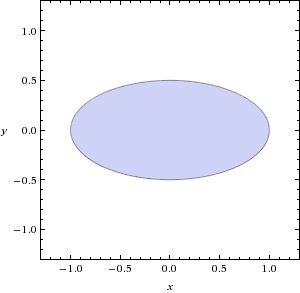
\includegraphics[width=6cm]{fig_8_4_2_a}
\captionof{figure}{}
\label{fig:8.4.2_a}
\end{minipage}

$E^\circ = \{(x,y):x^2+4y^2< 1\}$.

$\overline{\rm E} = E = \{(x,y):x^2+4y^2 \leq 1\}$.

$\partial E = \{(x,y):x^2+4y^2 = 1\}$.
\end{sketch}

\item
\begin{sketch} 
See the Figure \ref{fig:8.4.2_b}.

\begin{minipage}[h]{0.9\textwidth}
\centering
\definecolor{ffqqqq}{rgb}{1.,0.,0.}
\begin{tikzpicture}[line cap=round,line join=round,>=triangle 45,x=1.0cm,y=1.0cm]
\draw[->,color=black] (-1.,0.) -- (4.,0.);
\foreach \x in {-1.,1.,2.,3.}
\draw[shift={(\x,0)},color=black] (0pt,2pt) -- (0pt,-2pt) node[below] {\footnotesize $\x$};
\draw[->,color=black] (0.,-2.) -- (0.,2.);
\foreach \y in {-2.,-1.,1.}
\draw[shift={(0,\y)},color=black] (2pt,0pt) -- (-2pt,0pt) node[left] {\footnotesize $\y$};
\draw[color=black] (0pt,-10pt) node[right] {\footnotesize $0$};
\clip(-1.,-2.) rectangle (4.,2.);
\draw [line width=2.pt,color=ffqqqq] (1.,0.) circle (1.cm);
\draw [line width=2.pt,color=ffqqqq] (2.,0.)-- (3.,0.);
\end{tikzpicture}
\captionof{figure}{}
\label{fig:8.4.2_b}
\end{minipage}

$E^\circ = \phi$.

$\overline{\rm E} = E = \{(x,y):x^2-2x+y^2=0\}\cup\{(x,0):x\in[2,3]\}$.

$\partial E = E = \{(x,y):x^2-2x+y^2=0\}\cup\{(x,0):x\in[2,3]\}$.
\end{sketch}

\item
\begin{sketch} 
See the Figure \ref{fig:8.4.2_c}.

\begin{minipage}[h]{0.9\textwidth}
\centering
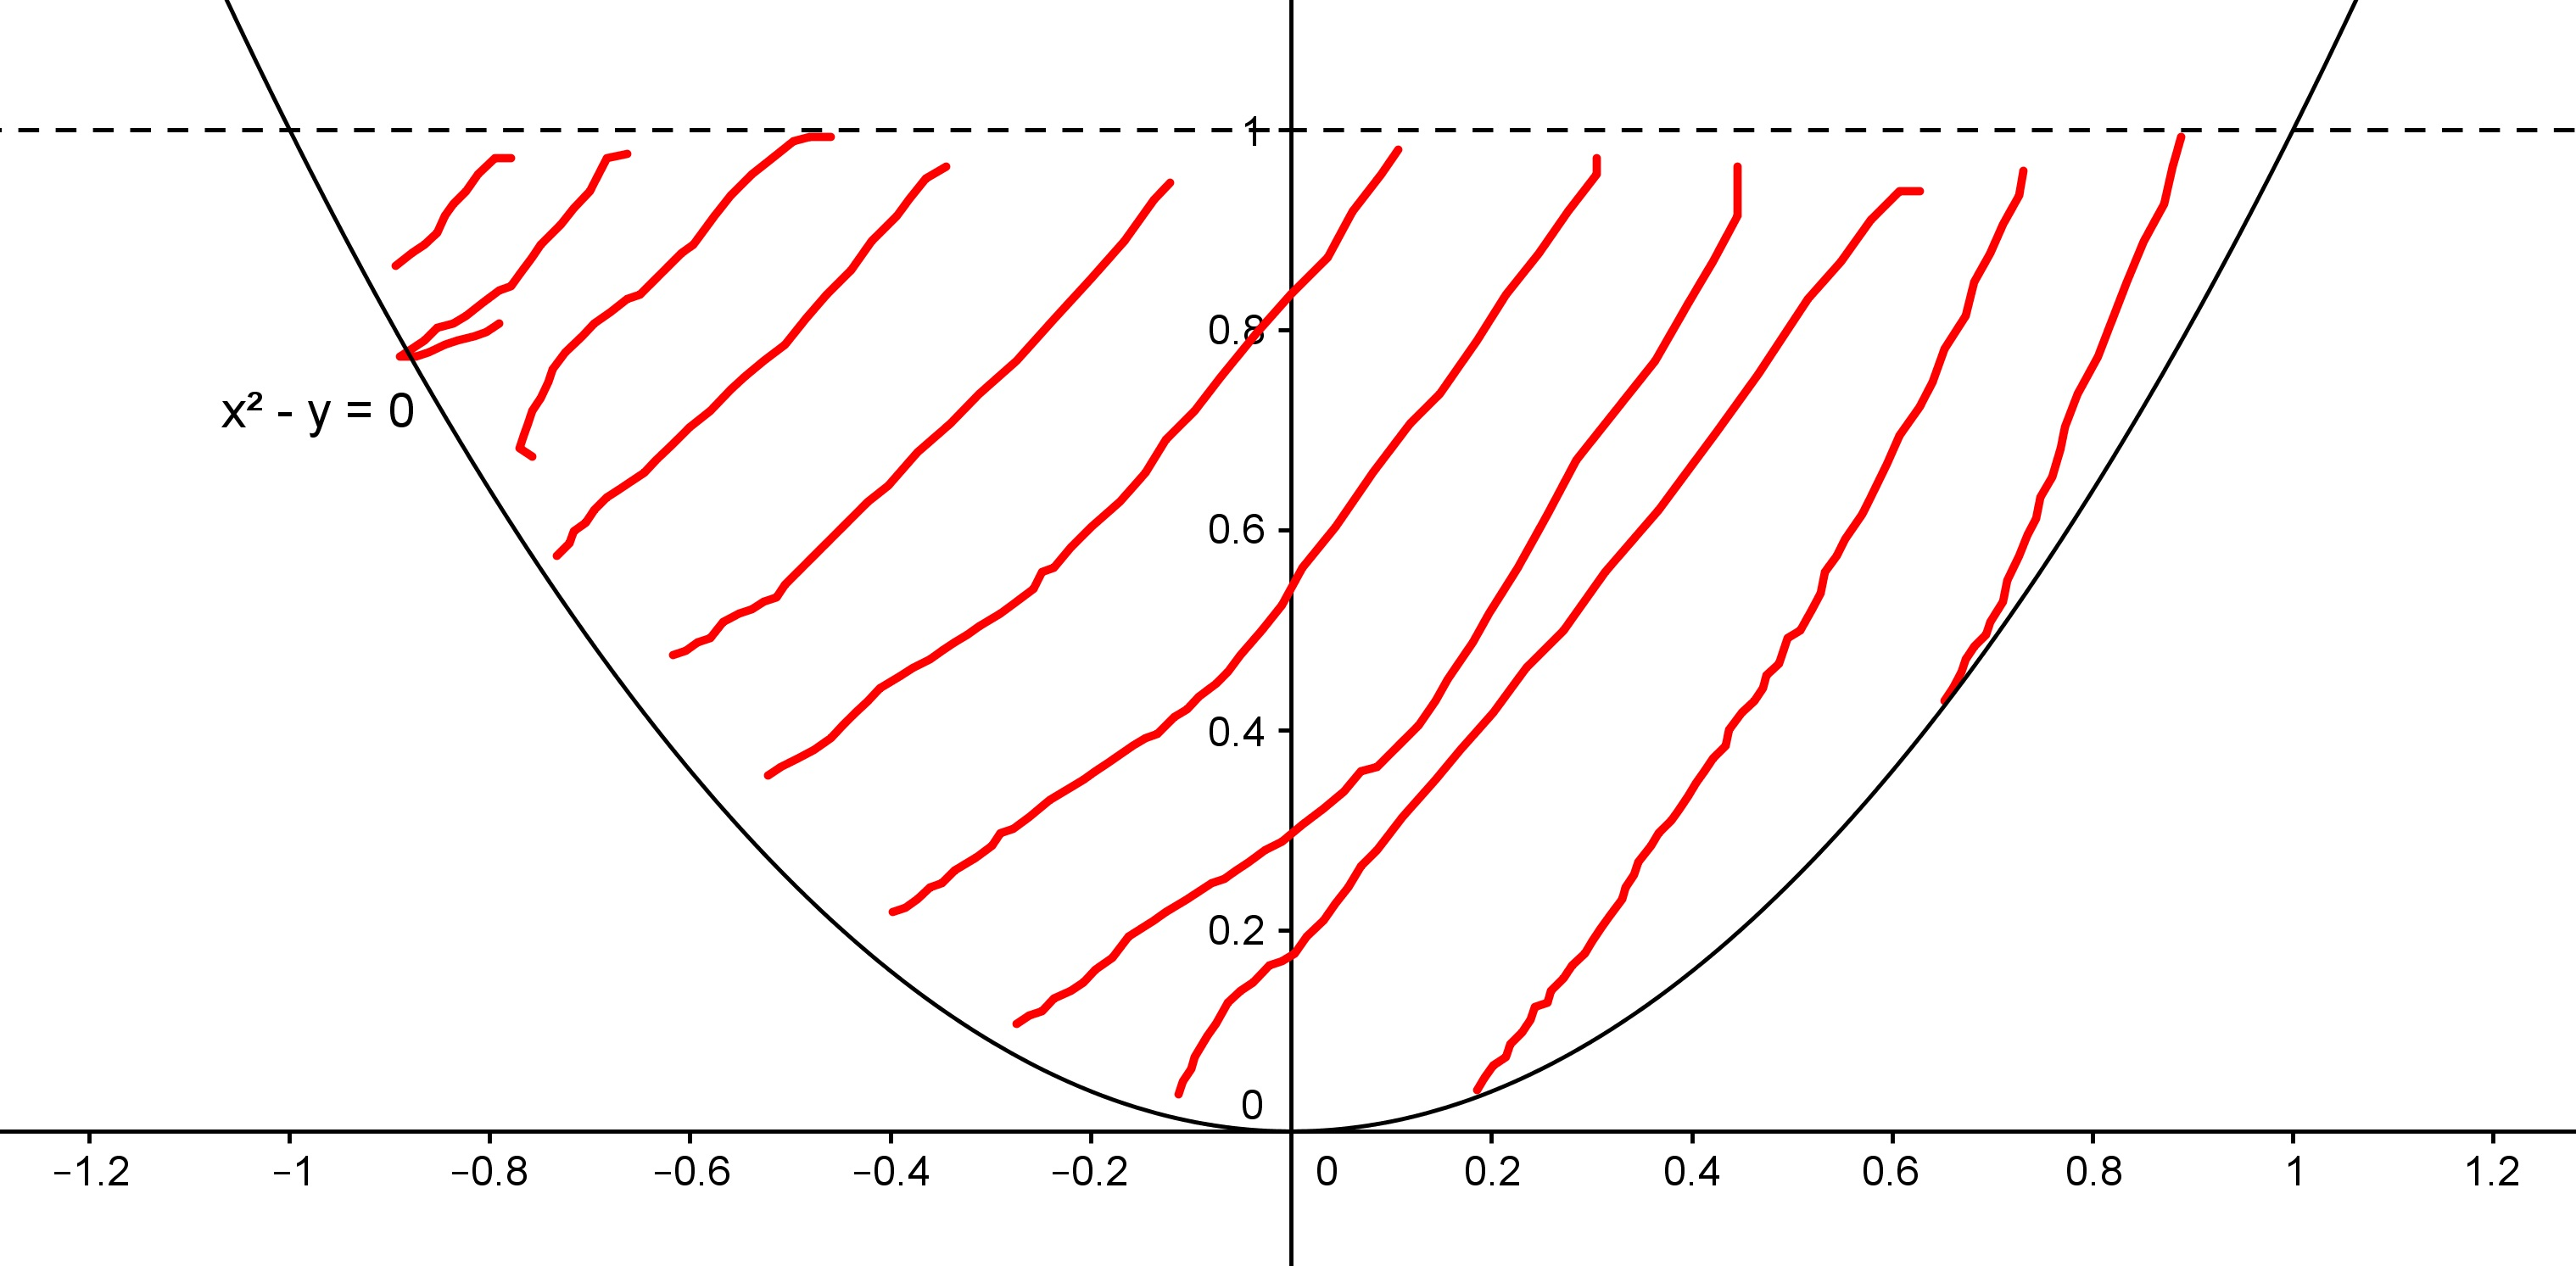
\includegraphics[width=0.7\textwidth]{fig_8_4_2_c}
\captionof{figure}{}
\label{fig:8.4.2_c}
\end{minipage}

$E^\circ = \{(x,y):y>x^2,0<y<1\}$.

$\overline{\rm E} = \{(x,y):y\geq x^2, 0\leq y \leq 1\}$.

$\partial E = \{(x,y):y=x^2,0\leq y \leq 1\}\cup\{(x,1):-1\leq x\leq 1\}$.
\end{sketch}

\item
\begin{sketch} 
See the Figure \ref{fig:8.4.2_d}.

\begin{minipage}[h]{0.9\textwidth}
\centering
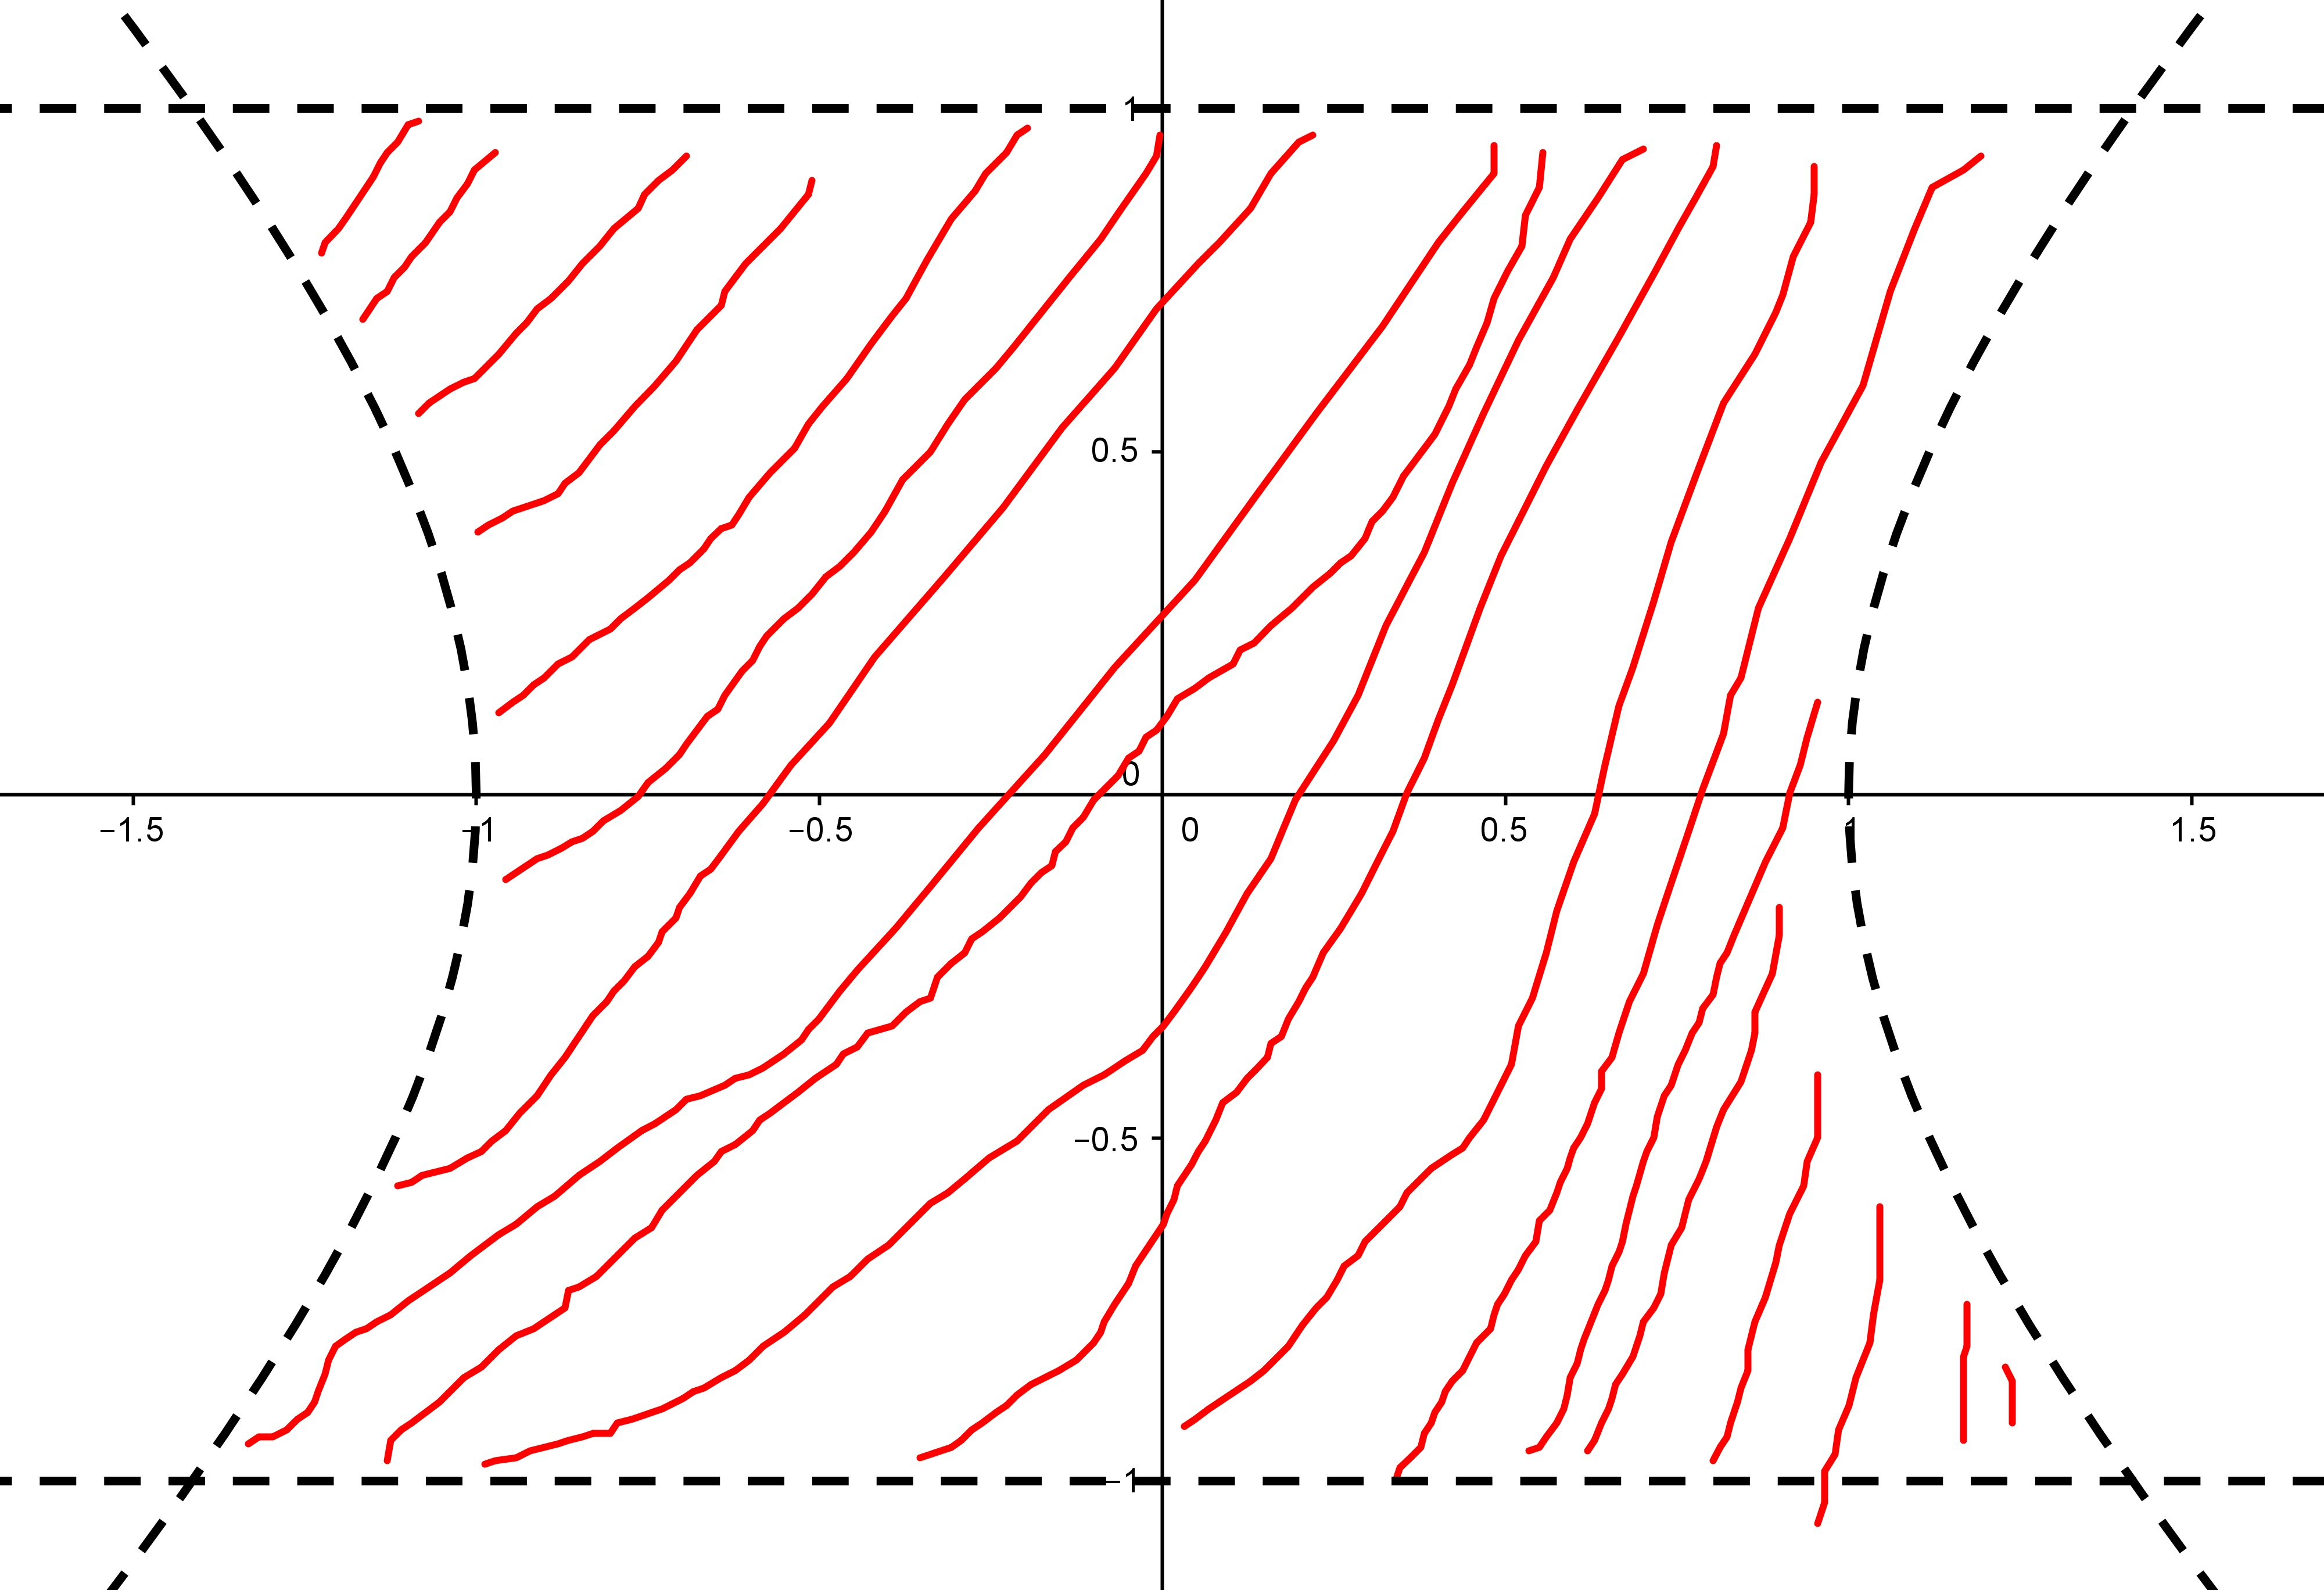
\includegraphics[width=0.7\textwidth]{fig_8_4_2_d}
\captionof{figure}{}
\label{fig:8.4.2_d}
\end{minipage}

$E^\circ = E = \{(x,y):x^2-y^2<1,-1<y<1\}$.

$\overline{\rm E} =  \{(x,y):x^2-y^2\leq 1,-1\leq y\leq 1\}$.

$\partial E = \{(x,y):x^2-y^2 = 1,-1\leq y\leq 1\} \cup \{(x,1):-\sqrt{2}\leq x \leq \sqrt{2}\} \cup \{(x,-1):-\sqrt{2}\leq x \leq \sqrt{2}\}$.
\end{sketch}

\end{enumerate}
\end{Exercise}

\vspace{12pt}

\setcounter{Exercise}{3}
% === Exercise 8.4.4 ===
\begin{Exercise}
\begin{enumerate}[a)]
\item
\begin{proof}
Let $$ B = \bigcup\left\{V:V\subseteq A, V\text{ is relatively open in }E\right\}.$$
It's clear that $B$ is relatively open in $E$.
\end{proof}

\item
\begin{proof}
Let $$ B = \bigcap\left\{V:V\subseteq A, V\text{ is relatively closed in }E\right\}.$$
It's clear that $B$ is relatively closed in $E$.
\end{proof}

\end{enumerate}
\end{Exercise}

\vspace{12pt}

\setcounter{Exercise}{5}
% === Exercise 8.4.6 ===
\begin{Exercise}
\begin{proof}
Since $E$ is connected, then we can suppose $a,b$ are extended real numbers, and discuss four situations as following.
\begin{enumerate}
\item [$\mathbf{Case\ 1.}$]
$E = (a,b)$

\item [$\mathbf{Case\ 2.}$]
$E = [a,b)$

\item [$\mathbf{Case\ 3.}$]
$E = (a,b]$

\item [$\mathbf{Case\ 4.}$]
$E = [a,b]$

\end{enumerate}

Then no matter the case is, we always conclude $E^\circ = (a,b)$ is an interval, so is connected.

\vspace{2ex}

If $\mathbb{R}$ is replaced by $\mathbb{R}^2$, we make $$E = \{(x,y):-1\leq x \leq 1, -|x| \leq y \leq |x|\},$$ then $$E^\circ = \{(x,y):-1 < x < 1, -|x| < y < |x|\}\backslash \{(0,0)\}$$ is not connected. Hence the proposition is false.
\end{proof}
\end{Exercise}

\vspace{12pt}

\setcounter{Exercise}{8}
% === Exercise 8.4.9 ===
\begin{Exercise}
\begin{enumerate}[a)]
\item 
\begin{solution}
Let $A=[0,1]$ and $B=(1,2]$, then
\begin{align*}
(A\cup B)^\circ &= (0,2) \\
A^\circ \cup B^\circ &= (0,1)\cup(1,2).
\end{align*}
Hence $(A\cup B)^\circ \neq A^\circ \cup B^\circ$.
\end{solution}

\item 
\begin{solution}
Let $A=[0,1]$ and $B=(1,2]$, then
\begin{align*}
\overline{\rm A\cap B} &= \emptyset \\
\overline{\rm A}\cap \overline{\rm B} &= \{1\}
\end{align*}
Hence $\overline{\rm A\cap B} \neq \overline{\rm A}\cap \overline{\rm B}$.
\end{solution}

\item 
\begin{solution}
Let $A=[0,1]$ and $B=(1,2]$, then
\begin{align*}
\partial (A\cup B) &= \{0,2\} \\
\partial A\cup \partial B &= \{0,1,2\}
\end{align*}
Hence $\partial (A\cup B) \neq \partial A\cup \partial B$. On the other proposition,
\begin{align*}
\partial (A\cap B) &= \emptyset \\
\partial A\cup \partial B &= \{0,1,2\}
\end{align*}
Hence $\partial (A\cap B) \neq \partial A\cup \partial B$.
\end{solution}

\end{enumerate}
\end{Exercise}
\end{document}
